\documentclass[11pt,twoside,openany]{report}
%\documentclass[10pt]{llncs}
%\usepackage{llncsdoc}
\usepackage{wrapfig}
\usepackage{lipsum}
\usepackage{amsmath,amssymb}
\usepackage{physics}
\usepackage{graphicx}
\usepackage{makeidx}
\usepackage{algpseudocode}
\usepackage{algorithm}
\usepackage{listing}
\usepackage{graphicx}
\usepackage{blindtext}
\usepackage{flafter}
\usepackage[bottom=0.75in,right=0.75in,left=0.75in]{geometry}
\usepackage{booktabs}   %% For formal tables:
                        %% http://ctan.org/pkg/booktabs
\usepackage{subcaption} %% For complex figures with subfigures/subcaptions
                        %% http://ctan.org/pkg/subcaption
\usepackage{enumitem}
% \usepackage{minted}
% \newminted{fortran}{fontsize=\footnotesize}

\usepackage{xargs}
\usepackage[colorinlistoftodos,prependcaption,textsize=tiny]{todonotes}

\usepackage{hyperref}
\hypersetup{
    colorlinks,
    citecolor=blue,
    filecolor=blue,
    linkcolor=blue,
    urlcolor=blue
}

\usepackage{epsfig}
\usepackage{tabularx}
\usepackage{latexsym}
\newtheorem{lemma}{Lemma}
\newtheorem{observation}{Observation}
\newtheorem{proof}{Proof}
\newtheorem{definition}{Definition}
\newcommand\ddfrac[2]{\frac{\displaystyle #1}{\displaystyle #2}}

\def\qed{$\Box$}
\def\proof{\textit{Proof. }}
\newtheorem{corollary}{Corollary}
\newtheorem{theorem}{Theorem}
\newtheorem{notation}{Notation}


\newcommand{\textbb}[1]{$\mathbb{#1}$}
\newcommand{\reals}{\mathbb{R}}
\newcommand{\levicevita}{\mathcal{E}}

% \newcommand\chapter{\if@openright\cleardoublepage\else\clearpage\fi
%                     \thispagestyle{plain}%
%                     \global\@topnum\z@
%                     \@afterindentfalse
%                     \secdef\@chapter\@schapter}

\title{Verified Computer Programs and Type Theory - A short report}
\author{Satyendra Kumar Banjare (16115102)}
\date{20-09-2018}

\begin{document}

\maketitle

\chapter*{Summary}

This is a report on advancements in type theory and formalized proof-based programming languages often referred to as verified programming languages. I have tried to explain the importance of mathematical modelling and logic system development based on the ancient works of mathematicians like Per-Martin Lof$^{1}$  by the applications in present programming toolchain and possible future aspects like applications in a quantum  programming toolchain.\\

Things are explained in chapter-wise manner and sufficient effort has been put to properly introduce things making understanding things easy.The chapters deal with mathematical logic systems first and then proceed to explain how this has been used and developed in real systems. With the current developments that are going on in this field, I have tried to explain the very possible usage in modelling a quantum computer's theoretical behaviour and applications in Machine Learning.\\

This area of study comes under the umbrella term of Programming Language Research and scientists all over have been  using these concepts to do explain the language semantics of any new programming language. This works using a system of inductive logics and as in abstract algebra, various operations on a given mathematical structure (\textit{example : Rings, Groups, Sets etc.}) a computer program is thought of being an operation on the a given type system. Type theory in its most literal meaning deals with the abstract idea of Types as a fundamental mathematical structures. Classical programming languages deals with data types and now some functional languages like \textit{Haskell, Agda, Ocaml etc} consider operations too as a type. Debugging has been made so easy because of the type systems and test driven development.\\

Consider the case where it is just some control signals flipping the states of bits and without a proper analytical typed contraint. The system's behaviour in this case will be completely unpredictable program-wise. Thus I would assume readers to believe with me that we would all like to have programs check that our programs are correct. Today most people who write software ,people from both academia and industry assume that the costs of formal verification of program outweighs the benefits. One simple example case is of \textit{javascript} programming language which is very informally developed thus has a very weak type system that often leads to bugs.  \textit{Haskell} on other hand does not allow programs to disobey the type system used for that program.\\ 



\tableofcontents


\chapter{Introduction and History }
\lipsum[1]
\lipsum[0]
\chapter{Abstract Algebra }

Abstract algebra \cite{abstractmaths} also referred to as modern algebra is the study of algebraic structures. An algebric structure serves as an explinatory basis of functional operations on an underlying set. A set here also is an abstract idea of a collection of things that share certain common features and should not only be confined with sets dealt in classical set theory. Over the time on the basis of types of operations and \textit{logical freedom} to do so on various sets have led to acceptance of various algebric structures defined below. The study of abstract algebra is used primarily in areas of topology of \textbf{n} dimensions. For anyone this is insane for physical boundations arise when we try to visualize things out. Thus we need to classify abstractions in one of the algebric structures and then deal with it. 

\section{Group Theory}

This is a part of abstract algebra where we deal with \textbf{Group} mathematical structures. In mathematics, a \textbf{Group} is an abstract algebraic structure that consists of a set of elements and various operations which when performed on any \textit{two} elements of the set results in a \textit{third} element from same set. It satisfies four conditions called the "group axioms" or "group properties", namely closure or closed operations i.e. that maps from set to itself , associativity, identity and invertibility. One of the most common examples of a group structure is the set of integers with the addition operation. This algebric structure is fundamental basis of other more complex algebric structures. It is studied in followings ways.\\

A group \textit{G} with the property with a given operation "o" such that \[ \textit{ a o b = b o a }  | \hfill \forall a,b \in \{ G \} \] is called abelian or commutative. Groups not satisfying this property are said to be nonabelian or non-commutative.

\subsection{Cyclic Groups}

A \textbf{Cyclic Group} is a group that can be generated by a single element often called as group generator). Cyclic groups are always Abelian. A cyclic group of finite group order n is denoted $G_n$ . The genralized generation rule can be specified as : \\

\[ X^n  = I ( X \in G ) \]

In the simple sense, it means identity element can be generated by any single element by repeated application of group operations. And since the identity element can be realized this way, all the elements of group can be realized too.\\

\subsection{Permutation groups}

A \textbf{Permutation Group} is a group G whose elements are permutations of a given set M and whose group operation is the composition of permutations in G (which are thought of as bijective functions from the set M to itself). The group of all permutations of a set M is the symmetric group of M, often written as Sym(M).[1] The term permutation group thus means a subgroup of the symmetric group. If M = {1,2,...,n} then, Sym(M), the symmetric group on n letters is usually denoted by Sn.

\subsection{Group Actions}

an action of a group is a formal way of interpreting the manner in which the elements of the group correspond to transformations of some space in a way that preserves the structure of that space.

. For other groups, an interpretation of the group in terms of an action may have to be specified, either because the group does not act canonically on any space or because the canonical action is not the action of interest. For example, we can specify an action of the two-element cyclic group \[ \displaystyle \mathrm {C} _{2}=\{0,1\}\] on the finite set \[\displaystyle \{a,b,c\}\] by specifying that 0 (the identity element) sends \[ \displaystyle a\mapsto a,b\mapsto b,c\mapsto c\], and that 1 sends \[ \displaystyle a\mapsto b,b\mapsto a,c\mapsto c \]. This action is not canonical.


\section{Field Theory}

In mathematics, a field is a set on which addition, subtraction, multiplication, and division are defined, and behave as the corresponding operations on rational and real numbers do. A field is thus a fundamental algebraic structure, which is widely used in algebra, number theory and many other areas of mathematics.\\
The best known fields are the field of rational numbers, the field of real numbers and the field of complex numbers. Many other fields, such as fields of rational functions, algebraic function fields, algebraic number fields, and p-adic fields are commonly used and studied in mathematics, particularly in number theory and algebraic geometry. Most cryptographic protocols rely on finite fields, i.e., fields with finitely many elements.\\
The relation of two fields is expressed by the notion of a field extension. Galois theory, initiated by Évariste Galois in the 1830s, is devoted to understanding the symmetries of field extensions. Among other results, this theory shows that angle trisection and squaring the circle can not be done with a compass and straightedge. Moreover, it shows that quintic equations are algebraically unsolvable.\\
Fields serve as foundational notions in several mathematical domains. This includes different branches of analysis, which are based on fields with additional structure. Basic theorems in analysis hinge on the structural properties of the field of real numbers. Most importantly for algebraic purposes, any field may be used as the scalars for a vector space, which is the standard general context for linear algebra. Number fields, the siblings of the field of rational numbers, are studied in depth in number theory. Function fields can help describe properties of geometric objects.\\

\section{Rings Theory}

In mathematics, a ring is one of the fundamental algebraic structures used in abstract algebra. It consists of a set equipped with two binary operations that generalize the arithmetic operations of addition and multiplication. Through this generalization, theorems from arithmetic are extended to non-numerical objects such as polynomials, series, matrices and functions.\\

Whether a ring is commutative or not (i.e., whether the order in which two elements are multiplied changes the result or not) has profound implications on its behavior as an abstract object. As a result, commutative ring theory, commonly known as commutative algebra, is a key topic in ring theory. Its development has been greatly influenced by problems and ideas occurring naturally in algebraic number theory and algebraic geometry. Examples of commutative rings include the set of integers equipped with the addition and multiplication operations, the set of polynomials equipped with their addition and multiplication, the coordinate ring of an affine algebraic variety, and the ring of integers of a number field. Examples of noncommutative rings include the ring of n × n real square matrices with n ≥ 2, group rings in representation theory, operator algebras in functional analysis, rings of differential operators in the theory of differential operators, and the cohomology ringof a topological space in topology.\\

\subsection{Polynomial Rings}

In mathematics, especially in the field of abstract algebra, a polynomial ring or polynomial algebra is a ring (which is also a commutative algebra) formed from the set of polynomials in one or more indeterminates (traditionally also called variables) with coefficients in another ring, often a field. Polynomial rings have influenced much of mathematics, from the Hilbert basis theorem, to the construction of splitting fields, and to the understanding of a linear operator. Many important conjectures involving polynomial rings, such as Serre's problem, have influenced the study of other rings, and have influenced even the definition of other rings, such as group rings and rings of formal power series.\\

A closely related notion is that of the ring of polynomial functions on a vector space. \\

\section{Iso-morphisms}

In abstract algebra, a group isomorphism is a function between two groups that sets up a one-to-one correspondence between the elements of the groups in a way that respects the given group operations. If there exists an isomorphism between two groups, then the groups are called isomorphic. From the standpoint of group theory, isomorphic groups have the same properties and need not be distinguished.


\section{Homo-morphisms}

In algebra, a homomorphism is a structure-preserving map between two algebraic structures of the same type (such as two groups, two rings, or two vector spaces). Homomorphisms of vector spaces are also called linear maps, and their study is the object of linear algebra.\\

% \section{Matrix Groups}

% In mathematics, a matrix group is a group G consisting of invertible matrices over a specified field K, with the operation of matrix multiplication, and a linear group is an abstract group that is isomorphic to a matrix group over a field K, in other words, admitting a faithful, finite-dimensional representation over K.\\

% Any finite group is linear, because it can be realized by permutation matrices using Cayley's theorem. Among infinite groups, linear groups form an interesting and tractable class. Examples of groups that are not linear include groups which are "too big" (for example, the group of permutations of an infinite set), or which exhibit some pathological behaviour (for example finitely generated infinite torsion groups). \\

% \section{Category Theory}

% Algebraic structures, with their associated homomorphisms, form mathematical categories. Category theory is a formalism that allows a unified way for expressing properties and constructions that are similar for various structures. \\

% The language of category theory is used to express and study relationships between different classes of algebraic and non-algebraic objects. This is because it is sometimes possible to find strong connections between some classes of objects, sometimes of different kinds. For example, Galois theory establishes a connection between certain fields and groups: two algebraic structures of different kinds.\\
\chapter{Computer Architecture}

\section{Instruction Set}
\section{Microarchitecture Design}
\section{Logic Synthesis}
\section{Implementation}
\chapter{Compilers}
\graphicspath{ {./images/} }


\textbf{Compilers}\cite{dragonbook} are that piece of software that \textit{translates} the programs in one language to other languages. They are different from \textbf{Assembler}. An assembler converts the assebly codes to final machines' instruction codes according to the ISA of the target computer hardware. Compilers are generally thought to convert higher level programs to low level programs. They are of different types like Cross compilers, Bootstrap Compilers (it comes under cross compilers)
, Transilers and De-compilers. The basic operations carried by most of the compilers are :\\

\section{Lexical Analysis}
This is the first part of any compiler that takes in the program spurce code and does word-substitutions, Macro expansions, generating \textit{Tokens} and cleaning up extra white spaces. All this work is done by using regular expression to increase compactness of input code. The tokens when combined in a special way form what is known as \textbf{Abstract Syantax Trees (AST)}. The regular expressions are interpreted as \textit{Non-Deterministic Finite Automata (NDFA)} since the states or the inner expression in between any two parts of a Regex can't be fixed since it will vary with the input used. Thus the NDFA is converted to \textit{Deterministic Finite Automata (DFA)} which will be parsed to AST using the technique of \textit{$\epsilon$-Transformation}.\\

\section{Syntax Analysis or Parsing}
This is the process of recombining the context-free grammatical tokens into a data structure, syntax tree. It is important that any sort of syntax error should be reported at this point of compilation. Context-free grammar is a recursive notation for describing sets of strings and imposing a structure on each such string \underline{without consiering the context in which the syntax is generated}.\\ 

\subsection{Abstract Syntax Trees and Abstract Binding Trees}
In computer science, an abstract syntax tree (AST), or just syntax tree, is a tree representation of the abstract syntactic structure of source code written in a programming language. It is "Abstract" in the sense that it does not represent every detail appearing in the real syntax of the programming language used, but rather just the structural and content-related details.\\

An abstract syntax tree is an ordered tree whose leaves are variables and whose interior nodes are operators whose arguments are its children. Ast’s are classified into a variety of sorts corresponding to different forms of syntax that divide ASTs into syntactic categories. For example, common programming languages often have a syntactic distinction between commands and an expression. These are two type of sorts for ASTs.\\

\textbf{Abstract Binding Trees (ABT)} enrich the meaning of AST with the methods to introduce new variables and symbols called \textit{bindings} to an existing AST. It should be noted that it is a theoretical concept and \underline{only AST is used in compilers while parsing}. The additions are performed within a given range of significance of the added terms called its \textit{scope}. In desinging type systems, we therefore deal with these ABT to construct new language.\\ 

Writing a new Programming language grammar basically involves writing syntactic sugar for \textit{Expressions, Statements }(often called commands) and \textit{Declaration} like header declarations and variable assisgnments. There are some \textbf{rules} defined and \textit{Judgements and derivations} are performed on them. The derivations are mostly inductive and also covers the finite aspect of machine. This can be understood in a way that DFA is mantained and machine never goes to a NDFA state.\\

For example here is a derivation of successor of a natural number, [ succ(succ(succ(zero)))nat ] : 

\[\dfrac{\dfrac{\dfrac{\dfrac{}{zero\quad nat}}{succ(zero) \quad nat}}{succ(succ(zero)) \quad nat}}{succ(succ(succ(zero))) \quad nat} \] .

The denominator in the expression is an inductive derivation from the numberator conditions.

\section{Type Checking}
This is one of the most important part where data consistency is checked of input source code. The Compiler may exploit or depend on type information, which makes it natural to combine calculation of types with the actual translation of source code. A language is considered to be type-safe if does not allow violation of basic data types. The varying level of strictness leads to formation of weak and strong type safe languages.\\

\begin{figure}[!htb]
\centering
  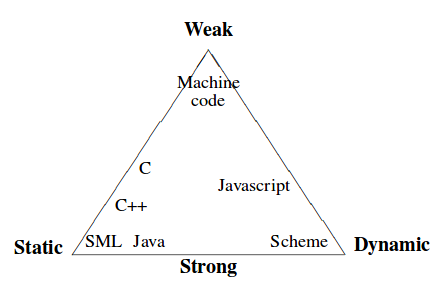
\includegraphics[scale=0.5]{type_check}
  \caption{Design Space of Types (source : Dragon book of compiler Technology)}
\end{figure}

It shows a diagram of the design space of static vs. dynamic and weak vs. strong typing, placing some well-known programming languages in this design space.

\section{Optimization}

This part deals with converting the present code as AST into more efficient using a series of transformations that makes the code use lesser sources but produces same output and variable scope is maintained throughout. Some of the common optimization techniques are :\\

\textbf{Peephole optimizations} replaces a complex multi-step instruction by an instruction of less-number of steps preferably a single step, for example multiplication by 2 is equivalent ot rotating bits to left by 1. \textbf{Data Flow Optimizations} convert expressions into simple to reduce number of duplicate expressions. \textbf{Static Single Assignment (SSA) optimization} involves assigning variables only a single value. If variables have same values then they are considered as one variable only. Scope Tables are used in these cases.

\section{Code Generation}
This part converts the optimized AST into machine codes of a hardware compatible ISA representation. It involves expoliting complex instructions and carefully placing jump and branch instructions for the machine code program. This part is also to be optimized and texhiques of \textit{Register allocation, Instruction selection, Instruction scheduling} and \textit{Rematerialization}. 

\section{Interpreter}
Interpreters are different from the compilers only in the aspect it performs operations as the code is produced without having a previously compiled code and then executing it. It works similar to a compiler in terms of basic steps but uses an \textbf{Interediate Representation (IR)} of AST before producing machine code and executing it too.\\

\textbf{Low Level Virtual Machine (LLVM)}\cite{llvm} is a popular compiler technology that takes into account the benefits of IR in compilation. It is used all over now and has increased portability of softwares a lot. Recently the \textit{Polyhedral Loop Optimizations (Polly)} in the LLVM IR has gained popularity and they have been used in all possible places.\\


\chapter{Type Systems}

A \textbf{Type System}\cite{typesystems} for any programming language is a set of rules that associate a property called "\textit{Type}" with the basic grammatical constructs of the language like variables, constants, statements and commands. It is the computer programming equivalent of type theory which uses type safety and type validation to prevent bugs, compiler runtime errors and compiler optimizations. It is very basic for any programming language to have types to actually perform any of \underline{Higher Order Logic} on the host machine. Note that a type system can work only if the program is run. In other words it is absolutely insignificant to check a program if it is not run or atleast compiled to be run.\\


%%%%%%%%%%%%%%%%%%%%%%%%%%%%%%%%%%%%%%%%
\section{Dependent Types }
\textbf{Dependent Types} \cite{dependent_types} is the most important kind of Types whose definition depends on a value. It is the conceptual overlap between computer's Type System and Type theory as it allows evaluation by induction. In functional Programming languages, dependent types increases expressivity of a defined type. It's examples include dependent functions and dependent pairs. Introduction of new variable or new values may completely change the overall behaviour. Thus the Structual Type checking would be used and not nominal (defined below). It is considered to be of two types from mathematical point of view : \\

\begin{itemize}
	\item{
	\subsection{ $\Pi$-Type}
	It is called \textbf{Dependent Product Type} where given a type space $\Omega$, we define a family of types B:A$\rightarrow$ $\Omega$ that says every term a:A has a type B(a):$\Omega$. It explains that there is not a fixed co-domain for functions of this type. The name 'pi-type' comes from the idea that these may be viewed as a Cartesian product of types. Pi-types can also be understood as models of universal quantifiers. For an example let's say a function gives tuple of order n for a given natural number input n. Clearly the terms in that tuple does not depend on the value of n. Here also, the Dependent product nature is preserved.\\   
	}
	\item{
	\subsection{ $\Sigma$-Type}
	It is called \textbf{Dependent Sum Type} and is \underline{categorically dual} to dependent product type where given a type space $\Omega$, if we have a family of types B:A$\rightarrow$ $\Omega$ then there must exist a dependent pair type. It explains that there should be fixed codomain for any function. \\ 
	}
\end{itemize}

They use mathematical operators ($\rightarrow$) and binders ($\forall$) to produce complex types. The higher order \textbf{Dependently Typed Polymorphic lambda calculus} also called \textbf{Calculus of Inductive Constructions} is the foundational basis of all Proof Assistants.

\section{Flow-Sensitive Types}
Such Type systems determine the type of a variable by controlflow. The type of a variable may change in any of the program's method. The type inference (defined below) is used for checking these type systems.

\section{Latent Types}
Latent typing refers to a type system where types are associated with values and not variables.

\section{Refinement Types}
These are a set of some preconditions that define the behaviour of the function or variable. These can be understood as the return types of most of functions which may dpend on some 'if/else' conditions.

\section{Substructural Types}
This is the type system defined depending on the use of a variable. For exmaple, a variable may be used once or many times. It has \textbf{Linear}, \textbf{Affine}, \textbf{Relevant} and \textbf{Ordered} as subcategories. The Linear system allows the use of object exactly once, Affine system allows use atmost once, Relevant system allows usage any number of times and Order system allows using objects only once in an order.

\section{Unique Types}
A Unique type guarantees that an object is used in a single-threaded way only with maximum one reference to it. It mantains the referntial transparency and improves the efficieny of functional languages.

%%%%%%%%%%%%%%%%%%%%%%%%%%%%%%%%%%%%%%%%%%%%%

\section{Type Safety \& Memory Safety }
Type safety refers to type equivalence and behavioural equivalence of all language constructs for a given program written in any programming language. Memory safety on the other hand refers to leakage and corruption of memory by any program. example : stack overflow.\\

%% Major Categories in Type Systems %%
Some Type checking techniques to ensure type safety are :

\begin{itemize} 
\item {\section*{Static vs Dynamic}

A \textbf{Static} type system refers to compilation time type checking. The source code's type correctness is verified first and then the executable is generated. A \textbf{Dynamic} type system checks type correctness during the runtime. This is the case when bindings and linking are created so that data passed on from one of the program to other is correct type-wise. Together both create polymorphic type checking where a single interface or a single Type check-pass is capable of doing both kind of type checks and is very portable to use. \\}

\item {
\section*{Nominal vs Structural}
In a \textbf{Nominal} or \textbf{Nominative} type system, the equivalence of data types is determined by explicit declarations or name of types. For example, in C programming language, two "\textit{struct} types with different names in the same translation unit are never considered compatible, even if they have identical field declarations. In \textbf{Structural} type system, the inner structure of a data type are evaluated  to show data equivalence and type safety. }

\item{
\section*{Manifest vs Inferred}
\textbf{Manifest} Typing is explicit identification by the software programmer of the type of each variable being declared. For example: if variable X is going to store integers then its type must be declared as integer. Type \textbf{Inference} refers to the automatic detection of the data type of an expression in a programming language. For example, user may write a float point decimal without having declared that variable as a float point. The compiler technology should be able to detect what program is trying to do and perform further actions accordingly. This is also referred to as \textbf{Typeless Typeing} where the type is later introduced depending on data passed.\\ }

\item{
\section*{Duck Type-ing}
This type system got it's name from on of the most common computer engineering practices which says if something behaves like a duck, quacks like aduck then it must be duck. In other words the behaviour determines the data type. For example, adding a float type integer to a double type integer, the answer should have a double type because it is surely to have characteristics of a double type integer.\\}

\end{itemize}

%%%%%%%%%%%%%%%%%%%%%%%%%%%%%%%%%%%%%%%%%%%%%
\section{Unified Type System}
In the object oriented programming (OOP) context, the abstraction and scope of methods deals with it's derivation from a base class. similar logic can be extended to class objects whose properties and methods depends on a base class. A \textbf{Unified Type System} states that all the Types of objects are derived from a single root type. Thus that object is capable of performing operations approved by the root type. Example of such a programming language is C\# developed by Microsoft.  In C\# the concepts of encapsulation and methods have been decoupled from the reference requirement so that a type can support methods and encapsulation without being a \textbf{Reference type}. A reference type is also an OOP concept that says all instances of class objects are by reference. \\


\chapter{Proving}
\lipsum[1]
\lipsum[0]
\chapter{Proof Assistants }
Having discussed some basic ideas of working of a Proof Assistant and theoretical soundness of proving things, let's now get to the programming and implementation. Proof Assistants as stated earlier is a software tool do help in developing formal proofs. As soon as the formal logic system was developed, a very basic theorem prover called  \textit{Logic for Computable Functions} (LCF) was developed along with a basic theoretical programming language \textit{Programming Computable Functions} (PCF) was developed. These were some of the initial works in the field of Proof Assistants. The successors include \textit{Isabelle} and \textit{COQ}. Also the theory advanced to reason for working at higher order of complexity called \textit{Higher Order Logics} (HOL).  


\section{LCF - Logic for Computable Functions}
This was the first interactive Automated theorem prover that also introduced a new \textit{Domanin Specific Language} (DSL) called ML. It allowed users to generate new tactics (disscussed below) to improve proving. The type system of ML ensures that theorems are derived completely by the given inference rules. \\

LCF shaped the thought process of how to write a type of a function to finally verify it by using terms like \textit{Inclusive} rules, \textit{Conditional} rules, \textit{$\lambda$} rules, \textit{Truth} rules. It also introduced the idea of tactic logics and put forward a \textit{Read Evaluate Print Loop} (REPL) type approach of proof assistant. It worked by breaking a given hypotheses into smaller forms. The smaller forms often are Lemmas on which the proof depends.\\

The  LCF-style  inference  kernel used in many proof assistants consists  of two layers: proof objects and theorems. Proof objects are represented as concrete datatypes. Depending on system parameters, a varying amount of information is maintained here. In any case, there is a complete record of oracles used in the proof. An explicit $\lambda$-term representation of the proof is also possible, but requires significantly more resources. Theorems are elements of an abstract datatype thm.\\

According to the original LCF tradition, theorems are proven propositions that have been certified by the kernel module, which implements primitive inferences as abstract datatype constructors. Any operation on theorems has to go through that kernel, so any value of type thm is “\textit{correct by construction}”.

\section{Tactics}
The forward reasoning of proving a hypothesis consisting of first proving sub-hypotheses say A and B and finally concluding that if A is proved and B is proved we have proved A\^B (our main hypothesis). The backward reasoing says to prove A\^B , we need to prove A and B. \textbf{Tactics} basically run inference rules forward or backwards to help break down proving things. It may also apply a predefined lemma ($\simeq$ function application), split up a lemma about some inductive type (in that particular step of proving) into a case for each constructor, and so on. \\

Basic tactics may succeed or fail depending upon the context in which they are applied. More advanced tactics are like little functional programs that run the basic tactics, perform pattern matching over the terms in the goal and/or assumptions, make choices based on the success or failure of tactics, and so forth. More advanced tactics deal with arithmetic and other specific kinds of theories. The key paper on Coq's tactic language is the following:

\section{De Bruijn criterion}
One may ask how to veify the verifying system being used. \textbf{De Bruijn criterion} answers this by ensuring that proof assistants create an ‘independently checkable proof object’ while the user is interactively proving a theorem. These proof objects should be checkable by a program that a skeptic user could easily write him/herself. De Bruijn’s Automath systems were the first to specifically focus on this aspect and therefore this property wascoined ‘De Bruijn criterion’ by Barendregt (Barendregt \& Geuvers 2001). In De Bruijn’s systems, the proof objects are basically encodings of natural deduction derivations that can be checked by a type checking algorithm.\\


\chapter{Programming Languages}
\lipsum[1]
\lipsum[0]
\chapter{Programming Language Verification }
\graphicspath{ {./images/} }

Any computer programming language consists of type system to its core supported by data structures and control flow techniques. Any Programming language finally can be broken down to machine codes resulting in perfoming specified actions. The assembly level machine codes should theoretically represent the same semantics as implied by the higher order programming language. \textbf{Programming Language Verification} in the broader sense is checking that programs in one programming language is equivalent to the one in other. Generally this equaivalence is tested between a high order	language and a small low level C language. \\

The basic understanding of how the verification work can be thought as, say there are two programs e$_1$ and e$_2$ then to prove they are equivalent the must meet the following criteria :

\begin{itemize}

\item{
	Input Parameters as well as the context in which the program is being run is same. Input parameters can be thougt as some initial values to a program. Input parameters should necessarily be of same type. The context refers to same harware used as well as the scope of the program in consideration is maintained same. Context can then again be broken as a \textit{Global} context and a \textit{Local} context. 
}

\item{
	The result should be same and should be of the same type. It is necessary that any program should not violate any of the bonding rules imposed by context.
}

\end{itemize}    

How do we check this ?\\

Well the method used is called \textbf{Step-Indexing}. In this method we look for holes in a program. These holes represented by C$_i$ can be thought as a program's loop structure or the way conditional arguments have been put up. In any step of a program thus if we are able to show that at that point, C$_2$[e$_1$] termminates and C$_1$[e$_2$] termminates also producing same results then we have shown the programs are equal. The cardinality issues related to number of such possible holes in programs increases the complexity of verification proof. This method therefore says that we should unfold the program upto required N steps and consider the equivalence then.\\

The areas where this method stucks is where we are unable to predict N. This is the case of IO type functions. The work on this is going on and improved proofs are being generated.\\


\section{Verified Software Toolchain}
This project led by Princeton University deals with verifying software programs and compilers. It is an advancement to Compcert. It uses multi layered kernels to securely verify the programs.  

\begin{figure}[!htb]
\centering
  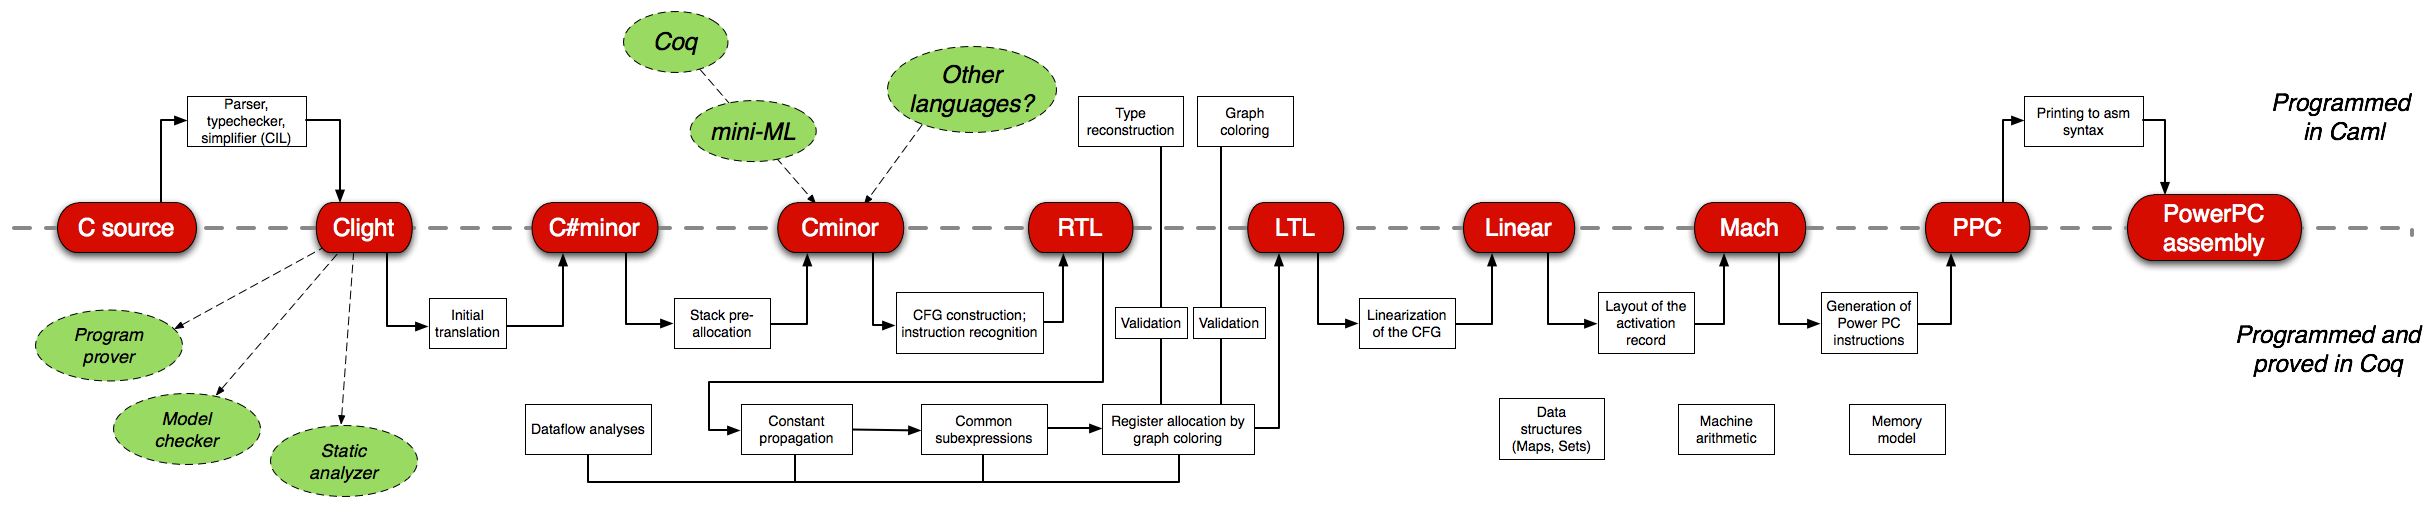
\includegraphics[width=\textwidth]{diagram}
  \caption{Flow diagram of CompCert C}
\end{figure}


\chapter{Complete Programming Stack Verification}
\graphicspath{ {./images/}} 

A computing programming stack being referred here is basically classical toolchain that includes all the tools from low level to high level. It includes compilers, linkers, debuggers, Database Management System (DBMSS) and interfacing kernels. The idea of stack verification is to check the correctness of all these technologies. Assuming the logical model of each of the software we can use the reasoning of Curry-Howard correspondence and Hoare Logic to construct a verifiable proof for each one.\\

\section{DeepSpec Project}


\begin{figure}[!htb]
\centering
  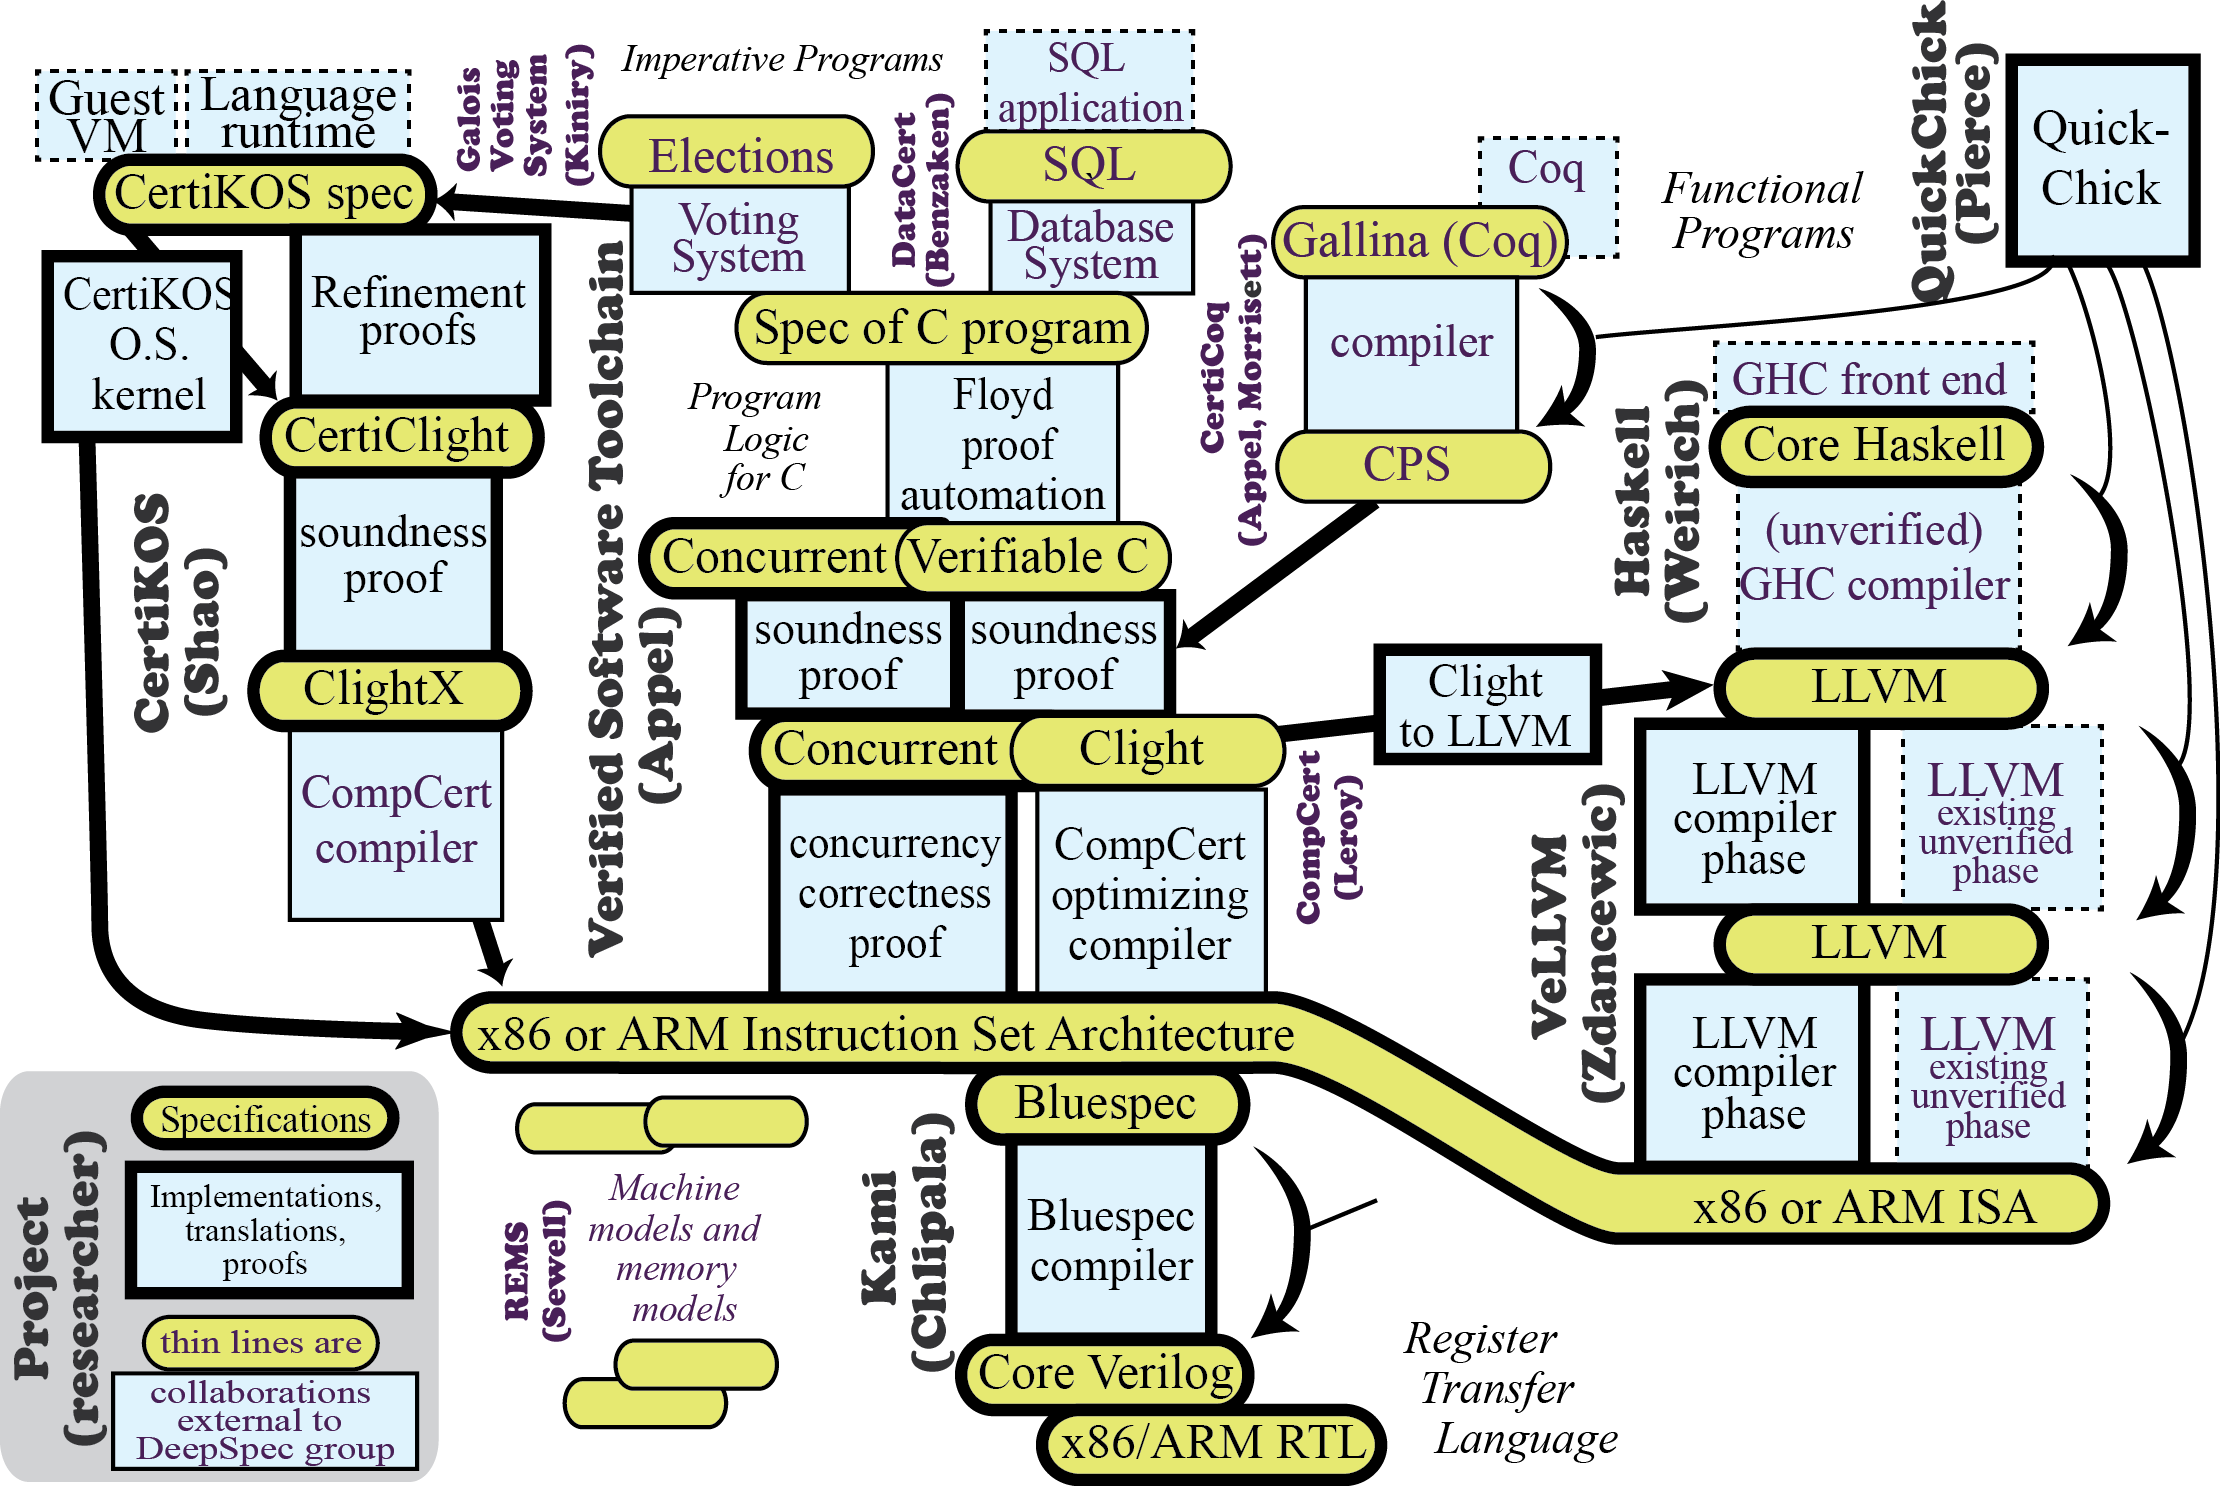
\includegraphics[scale=0.7]{deepspec}
  \caption{The DeepSpec Project}
\end{figure}

This project is umbrella project of many important projects like CertiCoq, VST, VELLVM, CertiKOS in the field of software verification. The subprojects deal with checking different software tools and also the operating system semantics. Thus the project DeepSpec overall verifies the computer stack. \\

A very basic explaination reads as provided in the manual, :

At the top of the diagram are specifications of application-level interfaces such as the semantics of the SQL query language or the rules governing fair Elections. At the bottom is the semantics of the RTL (register-transfer language) implementation of some specific microprocessor, say x86. A voting or database system is implemented as a C program with a specification Spec of C program, written in a program logic called Verifiable C. We prove (in Coq) that the C program correctly implements SQL by applying the program logic to the program, with the assistance of the Floyd proof automation system. Verifiable-C is a set of reasoning rules for program correctness; whatever properties are proved about a program will actually hold when the program runs; this is formalized in Coq as the soundness proof connecting Verifiable C to the operational semantics of C-light. The CompCert optimizing compiler compiles C light to machine language in ARM, PowerPC, or x86-ISA. The correctness of CompCert's translation is proved in Coq. Finally, the hardware is correct: the instruction set architecture x86-ISA is specified in the Bluespec hardware-description language, which itself has a deep specification defining its precise semantics. The Kami synthesizer translates this to register transfers written in Verilog (which, again, itself has a deep specification).\\

It would be a major breakthrough to completely build a coherent system of specified/verified components whose specification deals only with the semanics of some very basic technologies like for example Verilog and SQL.\\




\chapter{Quantum Computing Overview}
\graphicspath{ {./images/} }

\[ \boxed {\mbox{i\textbf{h}}\dfrac{\partial}{\partial t}|\psi(t)\rangle = \bm{\hat{\textnormal{\bfseries H}}} |\psi(t)\rangle }
\]

Quantum Computing is doing computation using quantum-mechanical phenomena like superposition and entanglement. A Quantum computer performs such computing and is very different from a classical computer that depends on digital logics and transistors. Quantum computation uses Quantum bits also called \textit{Qubits} which align in different ways to produce variations of not just 1 or 0 (as in classical computing) but many others. An approximation based on probability of outcome which depends on solving governing physics equations, theoretically allows us to construct subsequent logic of state or data changes.\\

A Quantum Turing Machine is theoretical accepted model of quantum computer which has been made possible by the initial works of \textbf{Richard Feynman}, \textbf{David Deutsch}  and \textbf{Yuri Manin}. The actual implemtation model of the quantum computer however is still in a very basic phase because of very absurd Temperature-Pressure conditions required to maintain a very less stable qubit state. The current research in quantum computing hardware focuses on precisely maintaining qubit's state and reducing data loss during state transition. The implementational software aspect of quantum computer is explored even smaller much because of less compatible quantum hardware and the inability of classical computers to simulate large qubit quantum computer.\\

\section{Qubits}
Quantum bits or Qubits are quantum version of classical binary bit. It is the basic unit of quantum information. Unlike the classical bits the Qubit can maintain information in unique states or in a superposition of states or may be  entangled states. The possiblity of having so many states improves the parallelism of data computaion and hence speed. A very good example is often potrayed by finding the card in which given 4 cards with one card different, we need to find the odd one out. The classical computer takes a maximum of 4 steps but a quantum computer will take always only 1 step to figure it out. 

\subsection{Representation}
Quantum State refers to the state of isolated quantum system. It gives a basic idea of possibility of different observable outcomes. A Qubit state can be represented by conventional "Dirac" or "bra-ket" notation, written as $|0\rangle$ or $|0\rangle$ and read as "ket-0" or "ket-1". two orthonormal \textit{Basis States} \{ $|0\rangle$ , $|1\rangle$ \} form 2-D linear vector space of qubit. Qubit basis states combine together to form \textit{Product Basis Space} like,

\[ |00\rangle = \begin{bmatrix} 1 \\ 0 \\ 0 \\ 0 \end{bmatrix} \quad \\
   |01\rangle = \begin{bmatrix} 0 \\ 1 \\ 0 \\ 0 \end{bmatrix} \quad \\
   |10\rangle = \begin{bmatrix} 0 \\ 0 \\ 1 \\ 0 \end{bmatrix} \quad \\
   |11\rangle = \begin{bmatrix} 0 \\ 0 \\ 0 \\ 1 \end{bmatrix} \quad \\
\]

A pure qubit state is a coherent superposition of the basis states. This means that a single qubit can be described by a linear combination of $|0\rangle$ \& $|1\rangle$.

\[|\psi\rangle = \alpha|0\rangle \quad +\quad \beta|1\rangle\]

with condition that 

\[\alpha^2 + \beta^2 = 1\ \cdots (i) \].

The probabilities of finding states of values $|0\rangle$ \& $|1\rangle$ is proportional to $|\alpha|^2$ and $|\beta|^2$ respectively.\\

The other type of representation is called \textbf{Bloch Sphere Representation} in which $\alpha$ and $\beta$ are considered as complex numbers with two degrees of freedom and a normalization constraint of equation (i). 

\begin{figure}[!htb]
\centering
  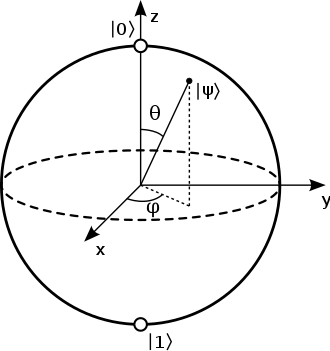
\includegraphics[scale=0.5]{bloch}
  \caption{Bloch Sphere Representation of a Qubit,}
\end{figure}

\[\alpha =  e^{i\psi}cos\dfrac{\theta}{2} \quad \& \quad \beta = e^{i(\psi + \phi)}sin\dfrac{\theta}{2} \].

\subsection{Quantum Superposition}
Superposition is essentially the ability of a quantum system to be in multiple states at the same time — that is, something can be “here” and “there,” or “up” and “down” at the same time.

\subsection{Quantum Entanglement}
It is a physical phenomena which that is said to occur when pairs or groups of particles are generated or they interact or share same spatial proximity such that behaviour of any one of the particles can not be defined independently of the state of others. Entanglement is an extremely strong correlation that exists between quantum particles — so strong, in fact, that two or more quantum particles can be inextricably linked in perfect unison, even if separated by great distances. The particles remain perfectly correlated even if separated by great distances. The particles are so intrinsically connected, they can be said to “dance” in instantaneous, perfect unison, even when placed at opposite ends of the universe. This seemingly impossible connection inspired Einstein to describe entanglement as "\underline{spooky action at a distance}".

\section{Quantum Gates \& Circuits}
A quantum gate or quantum logic gate is a rudimentary quantum circuit operating on a small number of qubits. They are the analogues for quantum computers to classical logic gates for conventional digital computers. \underline{Quantum logic gates are reversible}, unlike many classical logic gates. Some universal classical logic gates, such as the Toffoli gate, provide reversibility and can be directly mapped onto quantum logic gates. Quantum logic gates are represented by unitary matrices. The action of the gate on a specific quantum state is found by multiplying the vector which represents the state by the matrix representing the gate.\\


\begin{figure}[!htb]
\centering
  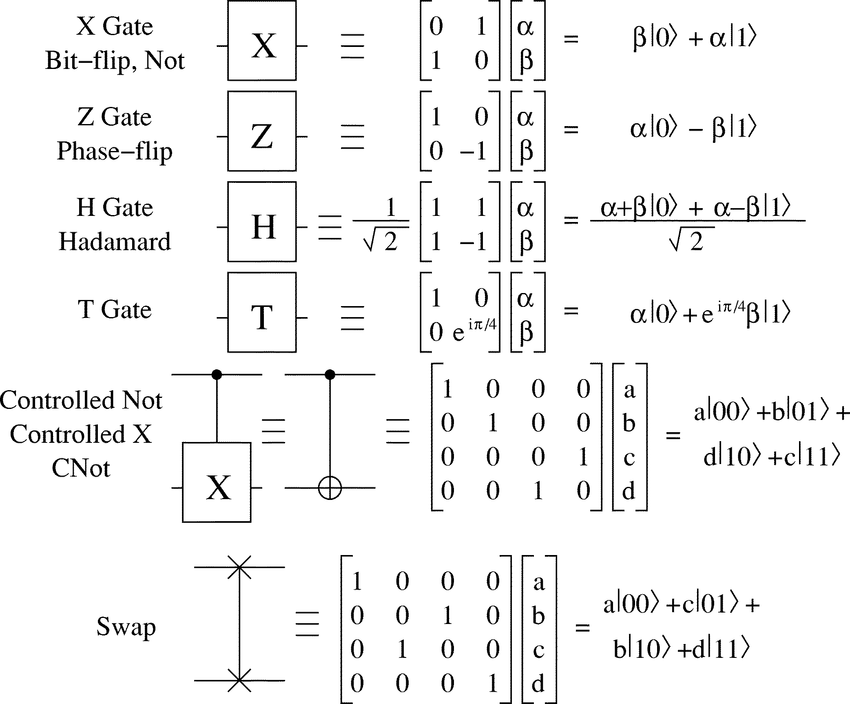
\includegraphics[scale=0.4]{qgates}
  \caption{Some common Quantum Logic gates}
\end{figure}

A \textbf{Quantum Circuit} is an ordered logical combination of quantum gates and some initial Qubits. The quantum circuits are reversible transformations on a quantum mechanical analog of an n-bit register. It is very important for any logic circuit to be reversible to return n bit data output for a n bit data input. In other words the reversible logic gates are bijective mappings from a n bit data set to itself. \textbf{Kitaev} \footnote{alphabeta} mentioned that irreversible circuits increase the physical entropy of the system. Theoretical advancements showed that \textbf{Toffoli Gate} is a Universal reversible Gate. this basically mean that we can easily consruct a large sizes circuit by simply adding more gates (Toffoli gates as example here) to it.

\begin{figure}[!htb]
\centering
  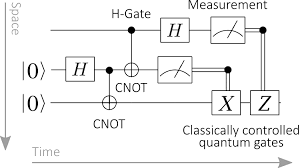
\includegraphics{qcircuit}
  \caption{An example of a quantum circuit}
\end{figure}

\subsection{Error Correction}
Error Corection is very important for scalibility of a quantum computer. An error correction of $10^{-2}$ means we can add atmost 100 logic gates before running into complete mess and even destroying the qubit chip. Research going on is trying to reduce this error correction to as low as possible.





\chapter{Quantum Computing Programming Languages}


\section{Quantum Computing SDKs}
\section{Imperative QC Languages}
\section{Functional QC Languages}
\section{Ongoing Development}
\chapter{Quantum Computing and Type Theory }
Programming languages are often recognized as Procedural and Descriptive corresponding to performing a given n-step logic in a program. Quantum Programs are verified throughly using Formal methods. A qubits working semantics are completely writtten as mathematical abstractions and then verified with some given initial conditions. Doing QC\footnote{Quantum computing} things this way is helpful as we are still not capable enough to have a practical quantum computer to try out things on. As in case of \textbf{Stack Verification} of classical computing systems, complete verification for quantum computers is also done. Some of the most recent works include \textit{Steve Zdancewic's} paper\cite{qwire} that discusses the \textbf{QWire} as a core language for Quantum circuits, an analogue to VHDL and HDL in classical computing. He has verified its correctness too in CoQ\cite{COQ}. He describes Phantom Types as the type system he used for Qwire.

\textbf{EpiQC}\cite{epiqc} is a multi-institutional paradigm foucsed on reducing the current gap between existing theoretical algorithms and practical quantum computing architectures. They have a very nice video series\cite{epiqc_video} that nicely explains the application of program verification in Quantum computing. They refer to Technology-Aware Programming Environment as an upgrade to traditional optimization and abstraction techniques to one that is more practical to use. Major focus is upon developing better tools for robustness and scalability.


\begin{itemize}
\item{
	\textbf{Procedural Implementations} include verifying step-by-step correctness of program semantics. \textbf{QCL} as described earlier is a programming language that has Procedural behaviour inherited from classical languages. It is now being verifed .   
}
\item{
	\textbf{Descriptive Implementations} involves verifying the program logic only. For example, a sum function should return summation of input parameters correctly. The procedural verification aspect of same would mean to check the register allocation and machine cycle logic verification. 
}
\end{itemize}

\section{Phantom Types}
Phantom Types \cite{phantom_types} is the  lightweight dependent type system used by Qwire. Most of the mathematical work involves matrices and using phantom types have increased the functional expressivity of the same. The complete implementation cna be found here 

\chapter{Applications in Machine Learning }
\lipsum[1]
\lipsum[0]

\chapter{Bibliography}
\lipsum[1]
\lipsum[0]

\end{document}

% \item Type theory - History \& Overview 
% \item Lambda Calculus
% \item Computer Architecture - Overview
% \item Compilers and Codegen
% \item Compiler Optimization
% \item Abstract Binding Trees \& Type System
% \item Imperative \& Functional Programming languages
% \item Embedded Languages \& untyped languages
% \item Proof Generation \& Proof Assistants
% \item Language Verificaton
% \item Quantum computing \& Qubits
% \item Quantum computing programming languages
% \item Advancements in Q\# and QASM
% \item Interplay of Type theory \& Quantum computing languages*
% \item Applications in Machine learning* 


% abstract-algebra.tex    book.cls                   history-and-introduction.tex  lec-4.tex  main.tex              proving.tex       stack-verification.tex
% abstract.tex            compilers.tex              interplay-qc-tt.tex           LICENSE    Makefile     qc-programming-languages.tex type-systems.tex
% applications-in-ml.tex  computer-architecture.tex  language-verification.tex     main.pdf   proof-assistants.tex  quantum-computing-overview.tex 
% programming-languages.tex
